\documentclass[draft]{cdr}
\pdfoutput=1            % must be in first 5 lines so arXiv finds it

% Edit: set this line to match this volume's sub-directories holding figures
\graphicspath{ {figures/}{volume-readme/figures/}{volume-readme/generated/} }

% Leave as is.
% This includes all common settings which are related to this
% particular CDR's set of volumes.
% This holds definitions of macros to enforce consistency in names.

% This file is the sole location for such definitions.  Check here to
% learn what there is and add new ones only here.  

% also see units.tex for units.  Units can be used here.

%%% Common terms

% Check here first, don't reinvent existing ones, add any novel ones.
% Use \xspace.

%%%%% Anne adding macros for referencing CDR volumes and annexes Apr 20, 2015 %%%%%
\def\expshort{DUNE\xspace}
\def\explong{The Deep Underground Neutrino Experiment\xspace}

\def\volintro{CDR Volume 1: Introduction\xspace}
\def\volphys{CDR Volume 2: Physics with DUNE at LBNF\xspace}
\def\vollbnf{CDR Volume 3: LBNF\xspace}
\def\voldune{CDR Volume 4: The DUNE Detectors\xspace}

\def\anxcernproto{Annex: CERN Single-phase Prototype Detector Proposal\xspace}
\def\anxlbnefd{Annex: LBNE FD Design Jan 2015\xspace}
\def\anxrates{Annex: Data Rates\xspace}
\def\anxndref{Annex: Near Detector Reference Design\xspace}
\def\anxlbnoa{Annex: LAGUNA/LBNO Part 1\xspace}
\def\anxlbnob{Annex: LAGUNA/LBNO Part 2\xspace}
\def\anxlbnesci{Annex: LBNE: Exploring Fundamental Symmetries of the Universe\xspace}
\def\anxdualrpt{Annex: Progress report on LBNO-DEMO/WA105 (2015)\xspace}
\def\anxdualtdr{Annex: WA105 TDR\xspace}

\def\cernsingleproto{Name of CERN Single-Phase Prototype\xspace}
\def\cerndualproto{Name of CERN Dual-Phase Prototype\xspace}

% Things about oscillation
%
% example: \dm{12}
\newcommand{\dm}[1]{$\delta m^2_{#1}$\xspace}
% example \sinstt{12}
\newcommand{\sinstt}[1]{$\sin^22\theta_{#1}$\xspace}
% example \deltacp
\newcommand{\deltacp}{$\delta_{\rm CP}$\xspace}
% example \nuxtonux{\mu}{e}
\newcommand{\nuxtonux}[2]{$\nu_{#1} \to \nu_{#2}$\xspace}
\newcommand{\numutonumu}{\nuxtonux{\mu}{\mu}}
\newcommand{\numutonue}{\nuxtonux{\mu}{e}}
\newcommand{\numu}{$\nu_\mu$\xspace}
\newcommand{\nue}{$\nu_e$\xspace}
\newcommand{\anumu}{$\bar\nu_\mu$\xspace}
\newcommand{\anue}{$\bar\nu_e$\xspace}

% Names
\newcommand{\cherenkov}{Cherenkov\xspace}
\newcommand{\kamland}{KamLAND\xspace}
\newcommand{\kamiokande}{Kamiokande\xspace}
\newcommand{\superk}{Super--Kamiokande\xspace}
\newcommand{\miniboone}{MiniBooNE\xspace}
\newcommand{\minerva}{MINER$\nu$A\xspace}
\newcommand{\nova}{NO$\nu$A\xspace}
\newcommand{\SURF}{Sanford Underground Research Facility\xspace}

\def\Ar39{$^{39}$Ar}
\def\driftvelocity{\SI{1.6}{\milli\meter/\micro\second}\xspace}


% Edit: set this to the subtitle specific to this volume
\renewcommand\thevolumesubtitle{Volume: README}

\begin{document}
% Leave as is. Initial content common to all volumes.
% This should be \input first thing after \begin{document}
\pagestyle{empty}

\begin{center}
  {\Huge  \thevolumetitle}

  \vspace{5mm}

  {\LARGE \thevolumesubtitle}
\end{center}


% Edit: input each chapter file in order

\chapter{Generalities}
\label{ch:generalities}

This volume gives guidance to authors and editors of the CDR volumes. It collects ``wisdom'' learned 
producing earlier documents, in particular the LBNE CDR and science document, and we will appreciate 
very much if everyone follows it!  It tries to follows its own guidance, so looking at its \LaTeX{} source can 
provide an example.  
%%%%%%%%%%%%%%%%%%%%%%%%%%%%%%%%%%%%%%%%%%%%%%%%%%%%%%%%%%%%%%%%%%%%
\section{Files}
\label{sec:files}

The entire CDR consists of a number of volumes, some of which are written in \LaTeX{}. These instructions apply only to the \LaTeX{} volumes.  You will find the \LaTeX{} and figure content for a given volume arranged like:

\begin{description}
\item[\texttt{volume-VNAME.tex}] the main file and is found in the top-level directory. It generally has no content itself but includes content through other files, some shared among the volumes and the bulk that makes each volume unique. 
\item[\texttt{figures/}] top-level subdirectory for any static figures shared by more than one volume
\item[\texttt{volume-VNAME/}] subdirectory holding all content for the volume
\item[\texttt{volume-VNAME/chapter-CNAME.tex}] holds the content for a chapter
\item[\texttt{volume-VNAME/figures/}] subdirectory holding any static volume-specific figures
\item[\texttt{volume-VNAME/generated/}] subdirectory holding any generated figures (see Section~\ref{sec:figures} for info on generated files)
\end{description}

Where \texttt{VNAME} is some label for the volume (this volume is called ``\texttt{readme}'') and 
\texttt{CNAME} is some label for the chapter (this current one is ``\texttt{general}'').  
Some general guidance:

\begin{itemize}
\item Do not include a volume number in the ``\texttt{NAME}'' nor a chapter number in ``\texttt{NAME}''.  The numbers will be determined by editors. 
\item Except for adding chapters to \texttt{volume-NAME.tex} please avoid any other changes to this file.   (the editors will probably take care of this anyway)
\item Use the \texttt{figures/} subdirectory for static figures (see Section~\ref{sec:figures}). For how to include generated figures see Section~\ref{sec:plots}.
\item If you find something inadequate or have questions, consult with either: \\
Anne Heavey, aheavey@fnal.gov, 630-840-8039 (technical editor)\\
Brett Viren, bv@bnl.gov (\LaTeX{}, graphics and git guru  -- so dubbed by Anne)
\end{itemize}

Files can get very big.  If they become unwieldy, we may want to separate out sections into 
separate tex documents and ``include'' them in the chapter document. Do this via an input 
statement, e.g.,
\begin{verbatim}
\input{chap-blah-section-blah}
\end{verbatim}

Even if your file isn't too long, please make it easier to navigate by using these long comment lines
to delineate the beginning of a new section, half the length for a subsection and a quarter the
length for a subsubsection.  

\begin{verbatim}
%%%%%%%%%%%%%%%%%%%%%%%%%%%%%%%%%%%%%%%%%%%%%%%%%%%%%%%%%%%%%%%%%%%%
\section{My Section}

%%%%%%%%%%%%%%%%%%%%%%%%%%%%%%%%%%%
\section{My Subsection}

%%%%%%%%%%%%%%%%
\section{My Subsubection}
\end{verbatim}


%%%%%%%%%%%%%%%%%%%%%%%%%%%%%%%%%%%%%%%%%%%%%%%%%%%%%%%%%%%%%%%%%%%%
\section{Figure Format}
\label{sec:figure-format}

It is essential to use high-quality, efficiently sized figures (aka ``graphics'').  You will be asked to redo 
them if they do not meet some basic standards.   
The standards are in place to avoid sub-optimal figures, bloated files sizes, and delayed publishing schedules.  

This section provides guidance on how to create figures 
according to the standards.

%%%%%%%%%%%%%%%%%%%%%%%%%%%%%%%%%%
\subsection{Graphic Types}
\label{sec:graphic-types}

There two basic graphic content types; these are important to understand:

\begin{description}
\item[raster] a two dimensional array of pixels
\item[vector] a two dimensional drawing description language
\end{description}

The CDR volumes compile with \texttt{pdflatex} and so can use graphics in PDF, JPEG or PNG file formats.  In general:

\begin{description}
\item[JPEG] use for photographs
\item[PDF] use of any line drawings, plots, illustrations
\item[PNG] use due to some inability to produce proper JPEG or PDF (contact editors)
\end{description}

It is possible (though unwise) to store inherently raster information in PDF or to rasterize inherently vector information into JPEG or PNG.  \textbf{This is the main cause for bloated, low-quality graphics.}  Here are some guidelines to avoid this:

\begin{itemize}
\item Only save photographic images to JPEG.
\item Save line drawings, plots or illustrations directly to vector PDF.
\item Follow special guidance on annotation (see Section~\ref{sec:annotate}).
\item Never convert any raster data (JPEG/PNG) to PDF.
\item Never raster what is really vector data in to a JPEG/PNG.
\item Never use MicroSoft PowerPoint for any figure as it tends to lead to poor quality and bloated files.
\item Do save using native application formats for later modification or conversion by experts.
\item Consider providing plots as ROOT, Python or other scripts.  (see Section~\ref{sec:plots})
\end{itemize}

\noindent If authors find these guidelines can not be followed, please contact the technical editors.   

%%%%%%%%%%%%%%%%%%%%%%%%%%%%%%%%%%
\subsection{Plots}
\label{sec:plots}

Where possible, it is recommended that any plots be submitted in a form that can be built along with the \LaTeX.  This allows editors to apply consistent in-plot fonts, colors, wording.  More info to be added.

%%%%%%%%%%%%%%%%%%%%%%%%%%%%%%%%%%
\subsection{Annotated Figures}
\label{sec:annotate}

One common figure type is to take a figure and annotate it with arrows or labels.  Ideally you will do this in 
LaTeX, for example using TikZ.  If you can't do that, then take care not to produce a bloated, low-quality graphic, and please choose fonts and colors that ``work'' with the document.  If the underlying graphic is JPEG then produce the final version in JPEG and never save as PNG.  If the annotation is on top of an original vector drawing and your annotation software will not raster it, save it as PDF.




\chapter{Writing \LaTeX}

This is the start of a chapter and gives some introduction before its first section.  This chapter describes basic \LaTeX{} you need to know.

%%%%%%%%%%%%%%%%%%%%%%%%%%%%%%%%%%%%%%%%%%%%%%%%%%%%%%%%%%%%%%%%%%%%
\section{Sectioning}
\label{sec:sectioning}

The following sectioning macros are available, ordered in descending
importance:

\begin{verbatim}
\chapter{A Chapter}
\section{A Section}
\subsection{A Sub Section}
\subsubsection{A Sub Sub Section}
\subsubsubsection{A Sub Sub Sub Section}
\end{verbatim}

Three-sub's is all you get.  
Consult with the technical editors if you feel finer grained
sectioning is required.
Starting from \verb|\subsection|, this produces the following:

\subsection{A Sub Section}
\subsubsection{A Sub Sub Section}
\subsubsubsection{A Sub Sub Sub Section}

Just after defining a chapter and any significant section a
\verb|\label| should be added so it can be referenced.
A label can be added later for a `'less significant'' section that
turns out to need one. You can label them all. 

For example:

\begin{verbatim}
\chapter{A Chapter}
\label{ch:a-chapter}

\section{A Section}
\label{sec:a-section}

\subsection{A Sub Section}
\label{subsec:a-subsection}
\end{verbatim}

See Section~\ref{sec:refs} for how to reference labeled sections.

\FloatBarrier
%%%%%%%%%%%%%%%%%%%%%%%%%%%%%%%%%%%%%%%%%%%%%%%%%%%%%%%%%%%%%%%%%%%%
\section{Figures}
\label{sec:figures}

See Section~\ref{sec:figure-format} for guidelines on the graphics files themselves.
Instead of using the usual \texttt{figure} environment a custom \texttt{cdrfigure}
environment is used in order to provide for a consistent presentation.
The environment is called with one optional and two required
arguments:

\begin{enumerate}
\item An initial, optional short caption for the List Of Figures, in square brackets.
\item A label for referencing (it will have \texttt{fig:} prepended). Curly brackets.
\item The full caption. Curly brackets, again.
\end{enumerate}

This is followed by including the graphic file.

\begin{cdrfigure}[Short ToF caption]{aerial}{An aerial photograph of Fermilab
    showing Wilson Hall and surrounding accelerator rings (Fermilab
    Visual Media Services)}
  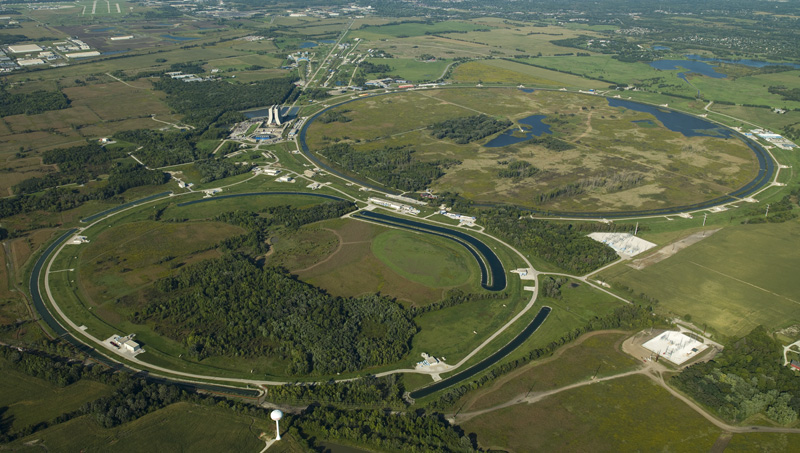
\includegraphics[width=0.8\textwidth]{fermilab-aerial.jpg}
\end{cdrfigure}


When the figure contains a graphic,  usually \texttt{includegraphics} is used.
The filename is assumed relative to a volume-specific \texttt{graphicspath} as
described in Section~\ref{sec:files} and as such one typically should
\textbf{not} specify any directory parts in its name.
The file's extension may be omitted.
An example can be seen in Figure~\ref{fig:aerial}, which is created
with the following \LaTeX shown in Figure~\ref{fig:aerial-latex}

\begin{cdrfigure}{aerial-latex}{\LaTeX{} showing how to do include a figure.}
\begin{verbatim}
\begin{cdrfigure}[Short ToF caption.]{aerial}{An aerial photograph of Fermilab
    showing Wilson Hall and surrounding accelerator rings (Fermilab
    Visual Media Services)}
  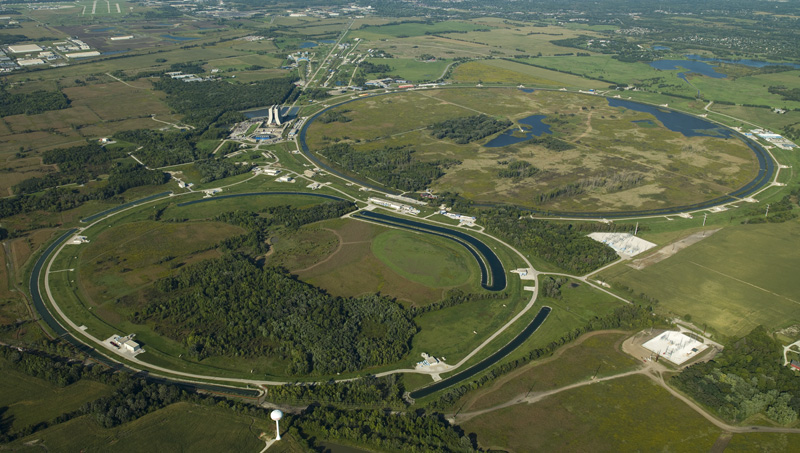
\includegraphics[width=0.8\textwidth]{fermilab-aerial.jpg}
\end{cdrfigure}
\end{verbatim}
\end{cdrfigure}

\FloatBarrier
%%%%%%%%%%%%%%%%%%%%%%%%%%%%%%%%%%%%%%%%%%%%%%%%%%%%%%%%%%%%%%%%%%%%
\section{Tables}
\label{sec:tables}

Like figures, we use a special environment, \texttt{cdrtable} for
tables to achieve a degree of consistency.
This is instead of the usual double \texttt{table} + \texttt{tabular} environments.
The \texttt{cdrtable} environment takes one optional and three
required arguments:

\begin{enumerate}
\item An initial, optional short caption for the List of Tables. Square brackets.
\item The tabular column specification. Curly brackets for the last three.
\item A label for referencing (it will have \texttt{tab:} appended)
\item The full caption.
\end{enumerate}

Inside the actual contents of the table you are required to provide a
initial row containing the headings for the table's rows followed by a
\texttt{toprowrule} macro.
Following every regular row (except the last) you should include a
\texttt{colline} macro.
Both of these take the place of the usual \texttt{hline}.

\begin{cdrtable}[The LoT caption]{cc}{example}
{This is an example table. We will use better colors, don't worry.}
  Rows & Counts \\ \toprowrule
  Row 1 & First \\ \colhline
  Row 2 & Second \\ \colhline
  Row 3 & Third \\ 
\end{cdrtable}

\noindent Table~\ref{tab:example} is thus made like (arguments can span lines):

\begin{verbatim}
\begin{cdrtable}[The LoT caption]{cc}{example}
{This is an example table. We will use better colors, don't worry.}
  Rows & Counts \\ \toprowrule
  Row 1 & First \\ \colhline
  Row 2 & Second \\ \colhline
  Row 3 & Third \\ 
\end{cdrtable}
\end{verbatim}

Table~\ref{tab:pdecay} shows a more complex example.
See the source for how it is written.
Note that special column specifications are used.

\begin{cdrtable}[Efficiencies and background rates for nucleon decay
  modes]{$L^c^c^c^c}{pdecay}{Efficiencies and background rates for
    nucleon decay channels of interest for a large underground LArTPC,
    and comparison with water Cherenkov detector capabilities} %$
  Decay Mode & \multicolumn{2}{^c}{Water Cherenkov} & 
\multicolumn{2}{^c}{Liquid Argon TPC} \\
\rowtitlestyle
& Efficiency & Background & Efficiency & Background \\ \toprowrule
$p \rightarrow K^+ \overline{\nu}$ & 19\% & 4 & 97\% & 1 \\ \colhline
$p \rightarrow K^0 \mu^+$ & 10\% & 8 & 47\% & $<2 $ \\ \colhline
$p \rightarrow K^+ \mu^- \pi^+$ & & & 97\% & 1 \\ \colhline
$n \rightarrow K^+ e^- $ & 10\% & 3 & 96\% & $<2$ \\ \colhline
$n \rightarrow e^+\pi^-$ & 19\% & 2 & 44\% & 0.8 \\
\end{cdrtable}

\FloatBarrier
%%%%%%%%%%%%%%%%%%%%%%%%%%%%%%%%%%%%%%%%%%%%%%%%%%%%%%%%%%%%%%%%%%%%
\section{Referencing and Citations}
\label{sec:refs}

Note: if you see a grey label blox containing \texttt{sec:refs}
between this paragraph and the section heading (or in general
elsewhere in chapters, sections, figures, etc), it means this document
was built in draft mode.  
These artifacts show up to help you know what label was used to
reference each particular thing.


\subsection{Intra-document References}

Assume that any chapter, section or important sub-, subsub-, section
or within any figure or table environment may need to be referenced
elsewhere in the text. As described in Section~\ref{sec:sectioning},
define a label (\verb|\label{...}| for these items.
Use the defined label in a \verb|\ref{...}| in order to make reference
to the chapter, section, figure, etc.
For example:

\begin{verbatim}
\chapter{Some Chapter}
\label{ch:some-chapter}

\subsection{Some Sub Section}
\label{subsec:some-sub-section}

...

As described in Chapter~\ref{ch:some-chapter} ...

As shown in Figure~\ref{fig:fermilab-aerial} ...
\end{verbatim}

When you reference a chapter, section, subsection, figure, table,
etc., capitalize the word ``Chapter'' or whatever it is, e.g., ``as
shown in Section~\ref{sec:plots}.''
Use the word ``Section'' even if it's a subsection or subsubsection,
and use the tilde sign to keep the number on the same line as the word
that precedes it.

Examples for figures and tables have been given above.  Here I
reference this section:~\ref{sec:refs}.  


\subsection{Citations}

Referencing citations is done like \verb|\cite{strunk}| which gives \cite{strunk}.
The key \texttt{strunk} matches an entry in the \texttt{common/citedb.bib}
file (as relative to the top-level directory).


The \texttt{citedb.bib} file is in BitTex format.
This is \textbf{not} \LaTeX{} format and in particular does not
indicate comments via \texttt{\%} characters.
The content and order of entries in this file is not reflected in the
generated Bibliography.
However, manual care must be taken to avoid duplication.
Before adding any entry to \texttt{citedb.bib} read/search through it
to ascertain that the entry you wish to add is not already there.








\chapter{Editing}

Some special facilities for editing the CDR are provided.


\section{Meta Markup}

While editing, it is possible to mark up the document with simple
\LaTeX{} macros as provided by the ``todonotes'' class.
This class has many features but a few are more important.



\subsection{Margin notes}

You can add notes to the \todo{run spell checker}margine easily which
are associated with some text using:

\begin{verbatim}
\todo{run spell checker.}
\end{verbatim}

\subsection{Highlighting}

If you wish to make add a comment on some section of text you may
\hlfix{highlight it}{This shows how.}
with a comment.


\begin{verbatim}
\hlfix{highlight it}{This shows how.}
\end{verbatim}


% \fixme[Anne]{CAN WE ADD THE FIXME BACK (OR EQUIVALENT?) AND TELL THEM ABOUT IT?}

\chapter{Technical}

This chapter describes some of the more technical aspects of the CDR.

%%%%%%%%%%%%%%%%%%%%%%%%%%%%%%%%%%%%%%%%%%%%%%%%%%%%%%%%%%%%%%%%%%%%
\section{Getting the Files and Compiling after your Changes}

Instructions for getting the files and compiling a volume are given on the home page of the repository, at
\href{https://github.com/LBNE/lbn-cdr}{https://github.com/LBNE/lbn-cdr}. Scroll down to 
``Guidance'' and ``Getting Started.''

Note that any acronyms list that a volume has requires an extra step to be included; this step
is not documented there.
The technical editors will take care of it.

%%%%%%%%%%%%%%%%%%%%%%%%%%%%%%%%%%%%%%%%%%%%%%%%%%%%%%%%%%%%%%%%%%%%
\section{The \LaTeX{} CDR class}

All of the \LaTeX{} configuration for the document that pertains to the general CDR style and not to the actual content is in the \texttt{cdr.cls} file.  The class takes some options that control high-level style:

\begin{description}
\item[\texttt{draft}] produce markup to assist in editing (line numbers, draft water mark, label tags)
\item[\texttt{print}] print quality (remove editing markup)
\end{description}

%%%%%%%%%%%%%%%%%%%%%%%%%%%%%%%%%%%%%%%%%%%%%%%%%%%%%%%%%%%%%%%%%%%%
\section{Volume-generic \LaTeX{} files}

There are several files specific to the topic of the CDR but used for all the volumes, hence 
they are in the \texttt{common} directory:

\begin{description}
\item[\texttt{common/preamble.tex}] placed before the document begins and should provide all macros to define common terms or units.
\item[\texttt{common/init.tex}] placed immediately after the document starts and should provide things like title page, author list, toc/lof/lot, etc.
\item[\texttt{common/final.tex}] placed immediately before the document ends and should provide the bibliography setup or any other common trailing matter.
\item[\texttt{common/defs.tex}] (input to the preamble) contains macros for some commonly 
used terms and expressions. Please review this file and use the definitions to help ensure consistency
throughout the document.
\end{description}

Also in the \texttt{common} directory are two content-related files: \texttt{intro.tex} and 
\texttt{supp-doc-list.tex}.  All volumes except the introductory volume will share the introduction
contained in \texttt{intro.tex}.  The other is a list of supporting documents that this
introduction file pulls in.

%%%%%%%%%%%%%%%%%%%%%%%%%%%%%%%%%%%%%%%%%%%%%%%%%%%%%%%%%%%%%%%%%%%%
\section{The volume-(name).tex file}

\hlfix{Contributors do not need to do this!} \\

To start a new volume, copy the \texttt{volume-readme.tex} to a new
name and edit as directed by the comments.  

\begin{enumerate}
\item Set the graphics path
\item Redefine the volumes sub-title
\item Input each chapter file.
\end{enumerate}



% Leave as is: Any final content common to all volumes.
% this is added just after end of document

\cleardoublepage

\bibliographystyle{ieeetr}
\bibliography{common/citedb}

\end{document}
